\section{FTable Converter}\label{ftableConverter}

FTable Converter

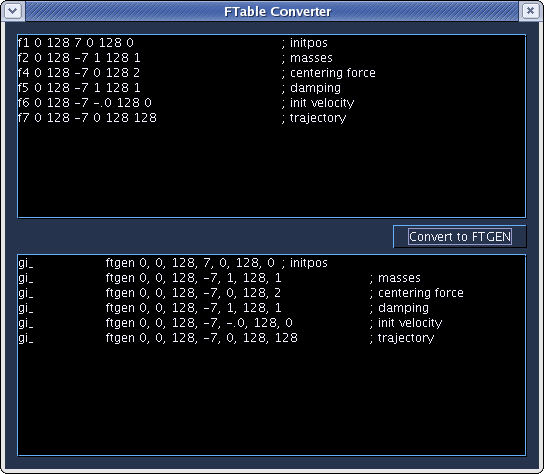
\includegraphics{images/ftableConverter.png}

The FTable Converter tool converts ftable statements into ftgen
statements. When converted, the prior ftable statement numbers are
ignored and ftgen statements are created using requested ftable number
of 0. The generated ftgen statements generate with the values of the
ftables set to "gi\_" with the expectation that the user will fill out
the rest of the name to be meaningful to them.

Conversion of ftable statements to ftgen statements is useful in
creating ftables that will be referenced by global variables instead of
hard-coded numbers.

To use, simply put your ftable statement text in the top text area and
press the "Convert to FTGEN" button to convert. For example, if you use
the following ftable statement text:

\begin{verbatim}
f1 0 128 7 0 128 0      ; initpos
f2 0 128 -7 1 128 1     ; masses
f4 0 128 -7 0 128 2     ; centering force
f5 0 128 -7 1 128 1     ; damping
f6 0 128 -7 -.0 128 0   ; init velocity
f7 0 128 -7 0 128 128   ; trajectory
\end{verbatim}

you will get the following output:

\begin{verbatim}
gi_ ftgen 0, 0, 128, 7, 0, 128, 0   ; initpos
gi_ ftgen 0, 0, 128, -7, 1, 128, 1    ; masses
gi_ ftgen 0, 0, 128, -7, 0, 128, 2    ; centering force
gi_ ftgen 0, 0, 128, -7, 1, 128, 1    ; damping
gi_ ftgen 0, 0, 128, -7, -.0, 128, 0  ; init velocity
gi_ ftgen 0, 0, 128, -7, 0, 128, 128  ; trajectory
\end{verbatim}

This work is based on the Steven Yi's FTable Converter web page utility
located \href{http://www.csounds.com/stevenyi/ftable.html}{here}.
